%================================================
% CHAPTER 1: GENERAL PROJECT FRAMEWORK
%================================================
\chapter{General Project Framework}

%================================================
\section{Introduction}

The rapid digital transformation of the banking sector is generating an unprecedented volume of
financial data, making effective data management and analytical decision-making increasingly
critical. Faced with dispersed, heterogeneous, and manually processed information, institutions
struggle to extract timely and actionable insights from their operational data.

It is within this context that this Final Year Project takes place, carried out over a
four-month internship (April to July 2025) at the \textbf{Arab Tunisian Bank (ATB)}. The
objective is to design and implement a comprehensive Business Intelligence solution that
automates data collection, structures it within a dimensional data warehouse, and delivers
interactive dashboards to support strategic and operational decision-making.

This chapter establishes the general framework of the project: a presentation of the host
institution, an analysis of the existing situation, a definition of the problem, and the
choice of the methodological approach.

%================================================
\section{Presentation of the Academic Institution}

International Tunis Business School (ITBS) is a private higher education institution
accredited by the Tunisian state. It distinguishes itself through a modern pedagogical
approach, focused on aligning training with the real needs of the job market, both nationally
and internationally.

ITBS offers high-quality programs in the fields of Management and Information Technology.
The Bachelor's degree in Management Information Systems (speciality Business Intelligence)
aims to train versatile professionals capable of designing complex information systems,
analyzing large volumes of data, and leading innovative Business Intelligence projects. It is
within the framework of validating this curriculum that this final year internship takes place.

\begin{figure}[H]
\centering

\includegraphics[height=2.5cm,keepaspectratio]{figures/download (1).png}
\caption{Logo of the International Tunis Business School (ITBS)\cite{itbs_logo} }
\label{fig:itbs_logo}
\end{figure}
\FloatBarrier

%================================================
\section{Presentation of the Host Organization}

\subsection{General Information}

Founded on June 30, 1982, from the integration of the Tunisian agency of Arab Bank Plc and
local capital, the \textbf{Arab Tunisian Bank (ATB)} is a Tunisian commercial bank. Since its
inception, the ATB has been committed to supporting the economic and financial development of
Tunisia by offering a wide range of high-quality banking services. Through a proactive business
development and management strategy inherited from Arab Bank, the ATB has positioned itself as
a key player in a competitive and constantly evolving banking market.

\begin{figure}[H]
\centering

\includegraphics[height=3cm,keepaspectratio]{atb_logo.jpg}
\caption{Logo of the Arab Tunisian Bank (ATB)\cite{atb_logo}}
\label{fig:atb_logo}
\end{figure}
\FloatBarrier

%------------------------------------------------
\subsection{Market Segments}

The ATB operates across several segments of the banking sector, each serving a distinct client
category:

\begin{itemize}
    \item \textbf{Retail Banking:} Services for individuals, including current accounts,
    savings accounts, consumer credit, bank cards (Visa, Mastercard), and digital services
    (ATBNet, ATBMobile).

    \item \textbf{Corporate Banking and Financial Services:} Financing solutions for
    businesses, including professional credits, leasing, treasury management, and trade
    finance (letters of credit, bank guarantees).

    \item \textbf{Credit and Savings:} Products such as real estate loans, auto loans,
    savings accounts, investment products, and contactless payment services (ATBPAY).
\end{itemize}

%------------------------------------------------
\subsection{Client Base}

The ATB serves a diversified client portfolio:

\begin{itemize}
    \item \textbf{Individuals:} Tailored banking products meeting personal financial needs.
    \item \textbf{Professionals and Enterprises:} Services including professional accounts,
    investment credits, and treasury management.
    \item \textbf{Large Institutions and Public Bodies:} Custom financial solutions designed
    to address specific and complex needs.
\end{itemize}

%------------------------------------------------
\subsection{Subsidiaries}

The ATB has several specialized subsidiaries:

\begin{itemize}
    \item Arab Financial Consultants (AFC)
    \item Arab Tunisian D\'{e}veloppement (ATD-SICAR)
    \item Arab Tunisian Invest (ATI-SICAF)
    \item Arab Tunisian Lease (ATL)
    \item AXIS Tr\'{e}sorerie (AT)
    \item CODIS
    \item SANADETT SICAV
    \item Soci\'{e}t\'{e} Arabe de R\'{e}alisations Immobili\`{e}res (SARI)
    \item Union de Factoring (Unifactor)
\end{itemize}

%------------------------------------------------
\subsection{Competitors}

The ATB operates in a competitive market, facing major players such as:

\begin{itemize}
    \item Banque BIAT
    \item Amen Bank
    \item STB Bank
    \item Zitouna Bank
\end{itemize}

%------------------------------------------------
\subsection{Agency Network and Workforce}

As of today, the ATB operates a network of more than \textbf{106 branches} across Tunisia
and employs more than \textbf{1,300 staff members}. In a context of rapid evolution of the
banking sector, the ATB has adopted a subsidiaries strategy, creating specialized entities to
diversify its services while maintaining solid relationships with both SMEs and large enterprises.

%------------------------------------------------
\subsection{ATB's Missions}

The ATB is committed to supporting the economic and financial development of Tunisia through
high-quality banking services. Its principal missions include:

\begin{itemize}
    \item Ensuring profitability, growth, and stability for shareholders.
    \item Consolidating its market position by meeting client expectations.
    \item Offering a motivating work environment that values respect and merit.
    \item Contributing to the country's economic and social development as a responsible
    corporate citizen.
\end{itemize}

%------------------------------------------------
\subsection{Organizational Structure}

The ATB's organizational structure is composed of the following entities:

\begin{itemize}
    \item \textbf{Central Directorate for Legal Affairs and Recovery:}
    Management of disputes and debt recovery.

    \item \textbf{Central Directorate for Risk Management:}
    Analysis and management of financial risks.

    \item \textbf{Compliance Directorate:}
    Verification of adherence to regulatory standards.

    \item \textbf{Central Directorate for Audit and Inspection:}
    Internal control and regularity verification.

    \item \textbf{Financial Division:}
    Supervision of financial operations.

    \item \textbf{Central Directorate for Credits:}
    Study and granting of credit facilities.

    \item \textbf{Central Directorate for Quality:}
    Improvement of services and procedures.

    \item \textbf{Information Systems Department:}
    Management of IT infrastructure and cybersecurity.

    \item \textbf{Central Directorate for Human Resources and Administrative Services:}
    Personnel management and logistics.

    \item \textbf{Central Directorate for Retail:}
    Development of the retail branch network.

    \item \textbf{Central Directorate for Corporate:}
    Management of corporate client relations.
\end{itemize}

\begin{figure}[H]
\centering
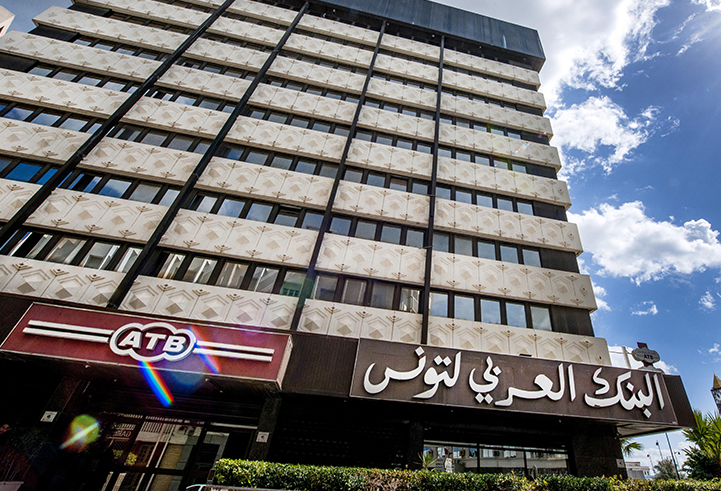
\includegraphics[width=0.75\textwidth]{atb_building.jpg}
\caption{ATB headquarters and organizational overview\cite{atb_logo}}
\label{fig:atb_logo}
\end{figure}
\FloatBarrier
%------------------------------------------------
\subsection{ATB Company Datasheet}

Table~\ref{tab:fiche_atb} presents the key factual information related to the host organization.

\begin{table}[H]
\centering
\renewcommand{\arraystretch}{1.6}
\caption{Arab Tunisian Bank (ATB) Company Datasheet}
\label{tab:fiche_atb}
\begin{tabular}{|p{5cm}|p{9cm}|}
\hline
\rowcolor{blue!15}
\textbf{Field} & \textbf{Details} \\ \hline
Full Name & Arab Tunisian Bank (ATB) \\ \hline
Date of Establishment & June 30, 1982 \\ \hline
Headquarters & 9 Rue H\'edi Nouira, 1001 Tunis, Tunisia \\ \hline
Phone & +216 71 351 155 \\ \hline
General Director & Riadh Hajjej \\ \hline
Share Capital & 128 million Tunisian Dinars \\ \hline
Commercial Register & B 167001997 \\ \hline
Branch Hours & Monday to Friday: 8:00--12:00 and 13:00--16:30 \\ \hline
Contact Email & qualite.retail@atb.com.tn \\ \hline
Website & \url{https://www.atb.com.tn} \\ \hline
LinkedIn & \url{https://www.linkedin.com/company/arabtunisianbank/} \\ \hline
\end{tabular}
\end{table}
\FloatBarrier

%================================================
\section{Project Presentation}

\subsection{Project Context}

This final year project, carried out as part of a four-month internship (April to July 2025)
at the ATB, validates the competencies acquired during the Bachelor's degree in Management
Information Systems, speciality Business Intelligence. It constitutes a key milestone towards
obtaining the diploma from ITBS.

Currently, the \textit{Direction March\'{e} Entreprises} of the ATB relies on a semi-automated
process for monitoring and controlling its commercial activities. Data is manually collected
from various sources and consolidated into Microsoft Excel spreadsheets to generate static
reporting dashboards. While this system offers a baseline level of reporting, it presents
significant limitations that hinder rapid and well-informed decision-making.

\subsection{Problem Statement}

The ATB's \textit{Direction March\'{e} Entreprises} currently relies on a manual data
consolidation process. Analysts collect records from multiple heterogeneous sources and
centralize them in Microsoft Excel files to produce static reporting dashboards.

Although this approach provides a baseline level of reporting, it exhibits significant
structural limitations:

\begin{itemize}
    \item Manual data entry is a frequent source of inaccuracies and inconsistencies.
    \item Static dashboards prevent interactive data exploration and drill-down analysis.
    \item The system cannot scale to handle growing data volumes efficiently.
    \item The reporting process is time-consuming and slows decision cycles.
    \item Limited decision reactivity reduces the speed and quality of strategic responses.
    \item The risk of analytical errors negatively impacts strategic choices.
\end{itemize}

The absence of a centralized and automated analytical infrastructure prevents optimal
exploitation of available data. It therefore becomes essential to design an intelligent,
automated system capable of consolidating, transforming, and visualizing data to support
rapid and evidence-based decision-making at the ATB.

\subsection{Project Objectives}

The primary objective of this project is to design a data management solution enabling rapid
and informed decision-making at the ATB. By aggregating and analyzing available data, this
solution aims to identify gaps between set objectives and achieved results, thereby facilitating
relevant strategic adjustments. The specific sub-objectives are:

\begin{enumerate}
    \item \textbf{Automated Data Ingestion Pipeline:} Design and deploy an automated ETL
    pipeline using \textbf{Airbyte} to extract data from heterogeneous operational sources
    and load it into a centralized staging area.

    \item \textbf{Data Warehouse and Dimensional Modeling:} Build a structured analytical
    data warehouse using a dimensional approach (star/constellation schema) hosted on
    \textbf{SQL Server} to enable multidimensional analysis and historical tracking.

    \item \textbf{Data Transformation Layer:} Implement a transformation layer using
    \textbf{dbt (data build tool)} to clean, model, and prepare data for analytical
    consumption, with full lineage tracking and documentation.

    \item \textbf{Pipeline Orchestration:} Deploy \textbf{Apache Airflow} to automate,
    schedule, and monitor the end-to-end data pipeline, ensuring reliability,
    observability, and fault alerting.

    \item \textbf{Customer Risk Scoring with Machine Learning:} Develop and integrate an
    \textbf{XGBoost}-based customer risk scoring model to classify clients by risk profile,
    enriching the analytical layer with predictive intelligence.

    \item \textbf{Interactive BI Dashboards:} Deliver a multi-page \textbf{Streamlit}
    dashboard enabling ATB managers and analysts to visualize KPIs, monitor commercial
    activity, and make data-driven decisions in real time.
\end{enumerate}

%================================================
\section{Study of the Existing System}

In order to design a relevant solution, an analysis of the tools currently used at ATB and
in the broader banking BI domain was conducted. Two tools are examined: Microsoft Excel,
the internal reporting tool used by the \textit{Direction March\'{e} Entreprises}, and
Microsoft Power BI, one of the most widely adopted external BI platforms. Since both tools
are part of ATB's analytical landscape, they are analyzed jointly below.

%------------------------------------------------
\subsection{Combined Analysis: Microsoft Excel and Microsoft Power BI}

\textbf{General Presentation}

The ATB's \textit{Direction March\'{e} Entreprises} currently uses \textbf{Microsoft Excel}
as its primary tool for data consolidation and reporting. Analysts manually collect data from
various operational systems and enter it into spreadsheets to produce reporting tables.
Alongside this internal practice, \textbf{Microsoft Power BI} --- one of the most widely
adopted Business Intelligence platforms in the industry --- serves as the external benchmark
for comparison. Power BI enables organizations to connect to multiple data sources, build
interactive dashboards, and share analytical reports across the organization via the cloud.

\begin{figure}[H]
\centering

\begin{minipage}{0.45\textwidth}
    \centering
    
\includegraphics[height=1.5cm]{excel_logo.png}
    \captionof{figure}{Microsoft Excel (ATB Internal Tool)\cite{excel_logo}}
    \label{fig:excel_logo}
\end{minipage}
\hfill
\begin{minipage}{0.45\textwidth}
    \centering
    
\includegraphics[height=1.5cm]{powerbi_logo.png}
    \captionof{figure}{Microsoft Power BI (Industry Benchmark)\cite{powerbi_logo}}
    \label{fig:powerbi_logo}
\end{minipage}

\end{figure}

\textbf{Detailed Analysis}

Table~\ref{tab:combined_analyse} presents a structured side-by-side analysis of both tools
across key BI dimensions.

\begin{table}[H]
\centering
\small
\renewcommand{\arraystretch}{1.3}
\caption{Combined analysis of Microsoft Excel and Microsoft Power BI}
\label{tab:combined_analyse}
\begin{tabular}{|p{3.5cm}|p{5.2cm}|p{5.2cm}|}
\hline
\rowcolor{blue!15}
\textbf{Aspect} & \textbf{Microsoft Excel (ATB Internal)} & \textbf{Microsoft Power BI (Industry)} \\ \hline
Data Collection & Manual entry from various operational sources & Automated connectors to 100+ data sources \\ \hline
Storage & Local or shared Excel files; no governance & Cloud-based or on-premise; role-based access \\ \hline
Processing & Formulas and pivot tables & DAX language for KPIs and calculated measures \\ \hline
Visualization & Static charts and tables & Interactive dashboards with drag-and-drop \\ \hline
Data Refresh & None; fully manual updates & Scheduled automated refresh \\ \hline
ML Integration & Absent & Limited; requires additional Azure ML services \\ \hline
Licensing & Included in Microsoft Office & High per-user licensing cost \\ \hline
\end{tabular}
\end{table}

Table~\ref{tab:combined_synthese} presents the combined strengths and weaknesses of both tools.

\begin{table}[H]
\centering
\small
\renewcommand{\arraystretch}{1.3}
\caption{Summary of strengths and weaknesses: Excel and Power BI}
\label{tab:combined_synthese}
\begin{tabular}{|p{3.5cm}|p{5.2cm}|p{5.2cm}|}
\hline
\rowcolor{blue!15}
\textbf{Dimension} & \textbf{Strengths} & \textbf{Weaknesses} \\ \hline
Microsoft Excel &
  Widely mastered; flexible for ad-hoc calculations; no infrastructure required; easy report sharing via email &
  Manual and error-prone; no versioning, lineage, or governance; static dashboards; not scalable \\ \hline
Microsoft Power BI &
  Intuitive interface; native connectors to many sources; automated refresh; widely documented &
  High licensing cost; cloud dependency; limited ML integration; restricted programmatic customization \\ \hline
\end{tabular}
\end{table}
\FloatBarrier

%================================================
\section{Synthesis of the Existing System Study}

The study of ATB's current Excel-based approach and the analysis of Power BI reveal a
strategic gap: on one hand, a fully manual, error-prone process with no scalability; on the
other, a proprietary BI platform that, while powerful for visualization, lacks native support
for custom ML integration and open-source pipeline orchestration. The solution developed for
ATB adopts a modern, open-source, data-driven architecture to address all these limitations:

\begin{itemize}
    \item \textbf{Data Automation:} Eliminates manual data collection
    through automated, scheduled ingestion pipelines.

    \item \textbf{Data Engineering:} Provides a structured,
    versionable, and documented transformation layer feeding a governed analytical warehouse.

    \item \textbf{Predictive Intelligence:} Complements descriptive BI with
    customer risk scoring, enabling proactive decision-making.

    \item \textbf{Interactive Dashboards:} Delivers fully customizable,
    programmatically controlled dashboards aligned with ATB's specific analytical needs.
\end{itemize}

%================================================
\section{Proposed Solution}
\label{sec:solution_proposee}

In response to the limitations of ATB's manual reporting process and the strategic gap
identified in the existing solutions study, we propose the design and implementation of a
\textbf{full-stack Business Intelligence and Machine Learning Platform}. This solution is
structured as a unified decision-support platform, organized across several coherent
functional and architectural modules.

\begin{figure}[H]
\centering
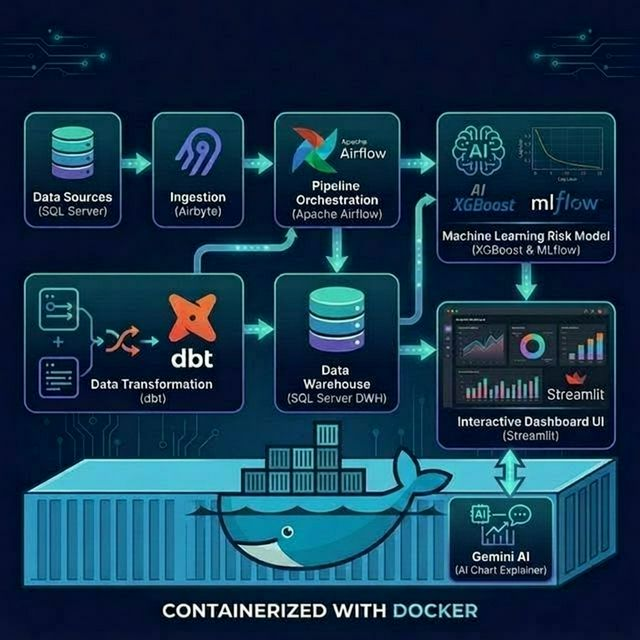
\includegraphics[width=0.92\textwidth]{figures/figure5.png}
\caption{Overview of the proposed Platform}
\label{fig:proposed_solution_overview}
\end{figure}
\FloatBarrier

\subsection{Functional Modules of the Solution}

The proposed solution is organized around a modular architecture ensuring automated
acquisition, structured storage, governed transformation, predictive enrichment, and
interactive restitution of data:

\begin{enumerate}
    \item \textbf{Automated Data Ingestion Module (Airbyte):}
    This component automates the extraction of data from heterogeneous operational sources
    and loads it into a centralized staging area. It resolves the data dispersion problem
    by consolidating raw information into a clean, normalized repository.

    \item \textbf{Data Warehouse and Dimensional Modeling (SQL Server):}
    To enable multidimensional analytical queries, the solution integrates a data warehouse
    modeled using a dimensional approach. This structure historizes facts related to client
    activities and risk while linking them to shared dimension tables representing clients,
    agencies, and time periods.

    \item \textbf{Data Transformation Layer (dbt):}
    The transformation layer uses \textbf{dbt (data build tool)} to apply business logic
    and quality rules to raw data. It produces clean, documented, and version-controlled
    analytical models with full data lineage.

    \item \textbf{Pipeline Orchestration (Apache Airflow):}
    The end-to-end data pipeline is orchestrated and monitored using \textbf{Apache Airflow}.
    DAGs (Directed Acyclic Graphs) schedule and coordinate ingestion, transformation, and
    ML scoring tasks, ensuring observability and controlled re-execution.

    \item \textbf{Predictive Scoring Engine (XGBoost):}
    At the core of the predictive layer, an \textbf{XGBoost}-based machine learning model
    scores customers by risk profile. Trained on historical behavioral and financial data,
    it classifies clients into risk categories, enriching the dashboards with proactive
    intelligence.

    \item \textbf{Decision Monitoring Interface (Streamlit Dashboard):}
    An interactive multi-page portal is made available to ATB managers and analysts. It
    provides dynamic visualization of KPIs, client risk distribution, agency performance,
    and temporal trends, enabling real-time data-driven decisions.
\end{enumerate}

\subsection{Functional Comparison with the Existing System}

Table~\ref{tab:comparatif_existant_solution} highlights the functional contribution of the
proposed solution compared to existing approaches.

\begin{table}[H]
\centering
\small
\renewcommand{\arraystretch}{1.5}
\caption{Functional Comparison: Existing Approaches vs.\ ATB BI Platform}
\label{tab:comparatif_existant_solution}
\begin{tabular}{|p{3.2cm}|p{3.3cm}|p{3.3cm}|p{4.3cm}|}
\hline
\rowcolor{blue!15}
\textbf{Criterion} & \textbf{Excel Reports} & \textbf{Power BI} & \textbf{ATB BI Platform} \\ \hline
Automation & Fully manual & Partial (scheduled refresh) & Daily automated pipeline (Airflow) \\ \hline
Data Model & None & Proprietary & Constellation schema (dbt + SQL Server) \\ \hline
Historical Tracking & Not supported & Limited & Time-versioned fact tables \\ \hline
Risk Analytics & Absent & Ad-hoc only & 3-pillar composite scoring model \\ \hline
ML Prediction & Absent & Custom visuals only & XGBoost + SHAP explainability \\ \hline
Interactivity & Static charts & Semi-interactive & Streamlit multi-page dashboard \\ \hline
Data Quality & Manual & No governance & Automated dbt tests \\ \hline
Reproducibility & Low & Low & Version-controlled pipeline \\ \hline
Licensing Cost & Included in Office & High per-user fee & Fully open-source \\ \hline
\end{tabular}
\end{table}

\subsection{Expected Benefits for ATB}

The deployment of this solution brings major strategic added value for the organization:

\begin{itemize}
    \item \textbf{Productivity and Automation:} Automated ingestion and transformation reduce
    data preparation time from hours to minutes, freeing analysts for higher-value tasks.

    \item \textbf{Standardization and Objectivity:} A governed, version-controlled data
    pipeline ensures consistent, auditable, and reproducible analytical outputs.

    \item \textbf{Proactive Predictive Intelligence:} The XGBoost risk model enables ATB to
    anticipate customer risk profiles rather than react to incidents.

    \item \textbf{Real-Time Decision Support:} Streamlit dashboards provide instant access
    to up-to-date KPIs, enabling management to monitor performance in real time.

    \item \textbf{Open-Source and Data Sovereignty:} The fully open-source stack eliminates
    vendor lock-in and licensing costs while keeping all data within ATB's infrastructure.
\end{itemize}

%================================================
\section{Project Methodological Framework}

\subsection{Comparison: Traditional vs.\ Agile Project Management}

Traditional project management relies on a sequential linear model (the waterfall cycle),
requiring exhaustive upfront planning structured into distinct successive phases. To clarify
the choice of methodology, Table~\ref{tab:comparaison_traditionnelle_agile} summarizes the
major differences between these two paradigms.

\begin{table}[H]
\small
\centering
\caption{Comparison of traditional and agile project management approaches}
\label{tab:comparaison_traditionnelle_agile}
\renewcommand{\arraystretch}{1.4}
\begin{tabular}{|p{2.8cm}|p{5.5cm}|p{5.5cm}|}
\hline
\rowcolor{blue!15}
\textbf{Characteristic} & \textbf{Traditional Approach} & \textbf{Agile Approach} \\
\hline
Project Structure & Sequential phases; each validated before advancing. & Iterative and incremental, favoring continuous adjustments. \\
\hline
Planning & Detailed upfront plan, difficult to change. & Adaptive planning evolving with the project. \\
\hline
Change Management & Changes are difficult and costly to integrate. & Changes are accepted and integrated fluidly. \\
\hline
Flexibility & Low; modifications are expensive mid-project. & High; rapid reactivity to evolving needs. \\
\hline
Communication & Formal, planned, and documented. & Continuous and collaborative within the team. \\
\hline
Deliverables & Fixed final deliverables, few intermediate revisions. & Frequent deliverable revisions at each iteration. \\
\hline
Testing & Tests performed at end of cycle. & Tests integrated at each iteration. \\
\hline
\end{tabular}
\end{table}

The comparative analysis highlights the significant advantages of the agile approach,
particularly in terms of flexibility, continuous collaboration, and adaptability.

%----------------------------------------------
\subsection{Comparison of Agile Methods: Scrum, Kanban, and XP}

Table~\ref{tab:comparaison_methodes_agiles} presents a comparison between the leading agile
frameworks.

\begin{table}[H]
\centering
\small
\caption{Comparison of agile methodologies}
\label{tab:comparaison_methodes_agiles}
\begin{tabular}{|p{2.8cm}|p{3.8cm}|p{3.8cm}|p{3.8cm}|}
\hline
\rowcolor{blue!15}
\textbf{Criteria} & \textbf{Scrum} & \textbf{XP} & \textbf{Kanban} \\
\hline
Planning & Start of each sprint with defined objectives & Planning games with team and client & Continuous Kanban-driven flow \\
\hline
Scope Changes & Integrated into next sprint & Continuous adaptation & Real-time priority adjustments \\
\hline
Key Roles & Scrum Master, Product Owner, Dev Team & Team and client & Team \\
\hline
Main Advantages & Productivity, scalability, team involvement & Code quality, reactivity & Quick setup, clear visualization \\
\hline
\end{tabular}
\end{table}

%----------------------------------------------
\subsection{Chosen Framework: Scrum}

In the context of this project, the \textbf{Scrum} framework was adopted as the overall
project management methodology. This agile approach, based on iterative and incremental
development, is well-suited to the evolving nature of requirements and the complexity of a
full-stack BI project.

Unlike rigid traditional methods, Scrum provides better visibility over progress, facilitates
mid-course adjustments, and encourages fluid communication through daily synchronization
points. The key advantages justifying this choice are:

\begin{itemize}
    \item Iterative, incremental, and adaptable approach.
    \item High responsiveness to changing requirements.
    \item Regular delivery of functional increments.
    \item Continuous improvement through retrospectives.
    \item Daily active team collaboration.
    \item Transparency in project tracking (backlogs, burndown charts)
    \item Reduced risk related to unforeseen changes.
    \item Better stakeholder satisfaction through frequent involvement.
\end{itemize}

%----------------------------------------------
\subsection{Scrum Roles}

The Scrum framework relies on three fundamental roles:

\begin{itemize}
    \item \textbf{Product Owner:} Representative of ATB stakeholders. Carries the product
    vision, defines and prioritizes functional requirements in the Product Backlog.

    \item \textbf{Scrum Master:} Guarantor of proper Scrum adherence. Removes impediments,
    facilitates collaboration, and protects the team from external disruptions.

    \item \textbf{Development Team:} Multidisciplinary team (data engineering, ML, BI) that
    is self-organized and responsible for delivering increments at each sprint.
\end{itemize}

%----------------------------------------------
\subsection{Scrum Artifacts}

\begin{itemize}
    \item \textbf{Product Backlog:} A prioritized and evolving list of requirements for the
    BI platform. Managed by the Product Owner.

    \item \textbf{Sprint Backlog:} A subset of the Product Backlog selected for a sprint,
    containing the objectives and tasks to complete.

    \item \textbf{Increment:} At the end of each sprint, a functional and deliverable result
    (e.g., an operational Airbyte pipeline, a validated dbt model, a deployed Streamlit
    dashboard).
\end{itemize}

%----------------------------------------------
\subsection{Scrum Events}

The sprint is structured by five key events:

\begin{itemize}
    \item \textbf{Sprint:} Fixed-duration iteration (2--4 weeks) producing a functional
    product version.

    \item \textbf{Sprint Planning:} Meeting defining the sprint objectives and selected items.

    \item \textbf{Daily Scrum:} 15-minute daily meeting sharing progress, plans, and blockers.

    \item \textbf{Sprint Review:} Demonstration of the completed increment to stakeholders.

    \item \textbf{Sprint Retrospective:} Analysis meeting to improve team practices.
\end{itemize}

These events create a collaborative, transparent, and value-delivery oriented framework.

%----------------------------------------------
\subsection{Comparison of Data Science Methodologies}

Well-structured data science methodologies are essential for the reproducibility and quality
management of analytical pipelines. Three major methodologies are compared in
Table~\ref{tab:comparaison_data_sciences}.

\begin{table}[H]
\small
\centering
\caption{Comparison of Data Mining and Machine Learning Methodologies}
\label{tab:comparaison_data_sciences}
\renewcommand{\arraystretch}{1.4}
\begin{tabular}{|p{2.5cm}|p{3.5cm}|p{3.5cm}|p{4cm}|}
\hline
\rowcolor{blue!15}
\textbf{Criteria} & \textbf{CRISP-DM} & \textbf{CRISP-ML(Q)} & \textbf{KDD} \\
\hline
Target & Generalist data mining & Machine Learning models & Large-scale databases \\
\hline
Advantage & Industry standard, well documented & ML-specific, integrates MLOps and QA & Proven for raw database exploration \\
\hline
Disadvantage & Ignores model drift in production & Requires mature MLOps infrastructure & Complex, technically demanding \\
\hline
\end{tabular}
\end{table}

%----------------------------------------------
\subsection{Chosen Tripartite Methodological Architecture}

At the conclusion of the comparative analysis, it became clear that no single method covers
all of the complex components of this project. A \textbf{tripartite methodological
architecture} was therefore adopted, where three methodologies are logically interlocked:

\begin{itemize}
    \item \textbf{Scrum (The Global Framework):} Used as the overall Project Management
    methodology, organizing the development calendar into 3 iterative Sprints structured as
    distinct functional and deliverable Releases.

    \item \textbf{CRISP-ML (The Technical Framework):} Used within Sprints dedicated to
    data engineering and machine learning, guiding ETL design, dimensional data warehouse
    modeling, XGBoost model training, MLOps tracking, and continuous monitoring.

    \item \textbf{GIMSI (The BI Business Framework):} Used within Sprints dedicated to
    dashboard development guiding KPI selection and visual design of decision-support
    interfaces for ATB management.
\end{itemize}

Table~\ref{tab:methodologie_tripartite} presents the tripartite methodological architecture.

\begin{table}[H]
\small
\centering
\caption{Tripartite methodological architecture of the ATB BI project}
\label{tab:methodologie_tripartite}
\begin{tabular}{|p{3cm}|p{4.5cm}|p{6.5cm}|}
\hline
\rowcolor{blue!15}
\textbf{Level} & \textbf{Methodology} & \textbf{Application in the Project} \\
\hline
Macro (Management) & Scrum & Global planning (3 Sprints/Releases), backlog tracking, incremental deliveries \\
\hline
Micro (Technical) & CRISP-ML & Airbyte ingestion, dbt transformation, DWH modeling, XGBoost training, MLflow tracking \\
\hline
Micro (Business) & GIMSI & Design and development of Streamlit dashboards for ATB management \\
\hline
\end{tabular}
\end{table}

The three following subsections detail each methodology and its concrete application.

%----------------------------------------------
\subsection{Data Science Methodology: CRISP-ML}

CRISP-ML (Cross-Industry Standard Process for Machine Learning) is a specialized, industry-standard
methodology designed to structure the end-to-end machine learning lifecycle. Unlike traditional data mining processes,
CRISP-ML explicitly incorporates MLOps requirements, quality assurance gates, experiment tracking, and continuous monitoring into six cyclical and iterative phases.

Figure~\ref{fig:crispml} illustrates the cyclic nature of the CRISP-ML methodology.

\begin{figure}[H]
\centering
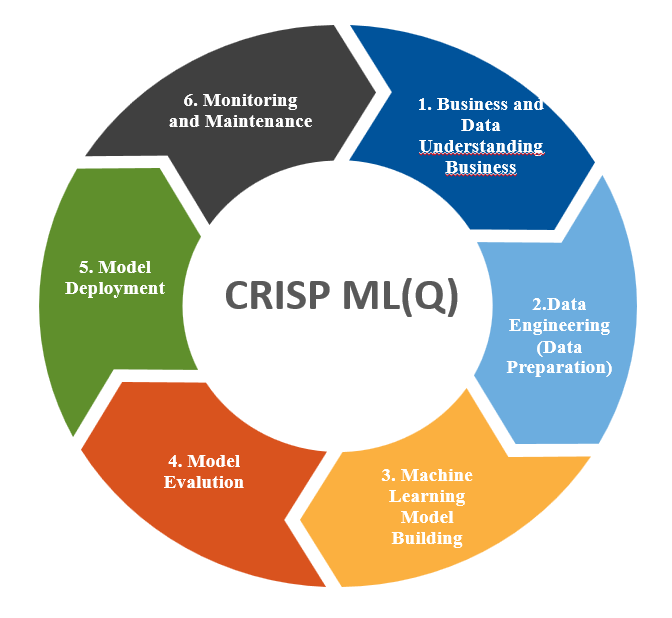
\includegraphics[width=0.42\textwidth]{crispml.png}
\caption{Cyclic representation of the CRISP-ML methodology\cite{crispml}}
\label{fig:crispml}
\end{figure}
\FloatBarrier

Table~\ref{tab:crispml_phases} presents the six phases of CRISP-ML and their concrete
application in the ATB BI project.

\begin{table}[H]
\small
\centering
\renewcommand{\arraystretch}{1.5}
\caption{The 6 phases of CRISP-ML applied to the ATB BI project}
\label{tab:crispml_phases}
\begin{tabular}{|c|p{4cm}|p{7.5cm}|}
\hline
\rowcolor{blue!25}
\textbf{Phase} & \textbf{CRISP-ML Phase Name} & \textbf{Application in the ATB Project} \\
\hline
1 & Business \& Data Understanding & Defining \textit{Direction March\'{e} Entreprises} operational goals, risk scoring requirements, and evaluating data source availability \\
\hline
2 & Data Engineering \& Preparation & Ingestion via Airbyte, cleansing and transformation via dbt into DWH, leakage-free feature engineering (34 indicators) \\
\hline
3 & ML Model Engineering & XGBoost customer risk scoring model training, hyperparameter optimization, MLflow experiment tracking \\
\hline
4 & Quality Assurance \& Evaluation & Performance validation against quality gates (F1 $\geq 0.70$, ROC-AUC $\geq 0.80$), confusion matrix, SHAP explainability \\
\hline
5 & Model Deployment & Promotion in MLflow Model Registry, integration into Streamlit dashboard (\textit{ML Risk Intelligence}), interactive risk predictor \\
\hline
6 & Model Monitoring \& Maintenance & Airflow orchestration (\texttt{dag\_ml\_pipeline}), automated batch scoring into DWH, disagreement alerting \\
\hline
\end{tabular}
\end{table}
\FloatBarrier

%----------------------------------------------
\subsection{Application of Scrum to Project Development}

The iterative nature of the ATB BI project, characterized by evolving data requirements and
incremental deliverable validation by ATB stakeholders, makes the classical cascade approach
unsuitable. The Scrum framework organizes work into fixed-duration Sprints (three to four
weeks), structured into functional and deliverable Releases.

Figure~\ref{fig:scrum} illustrates the Scrum development cycle applied to this project.

\begin{figure}[H]
\centering
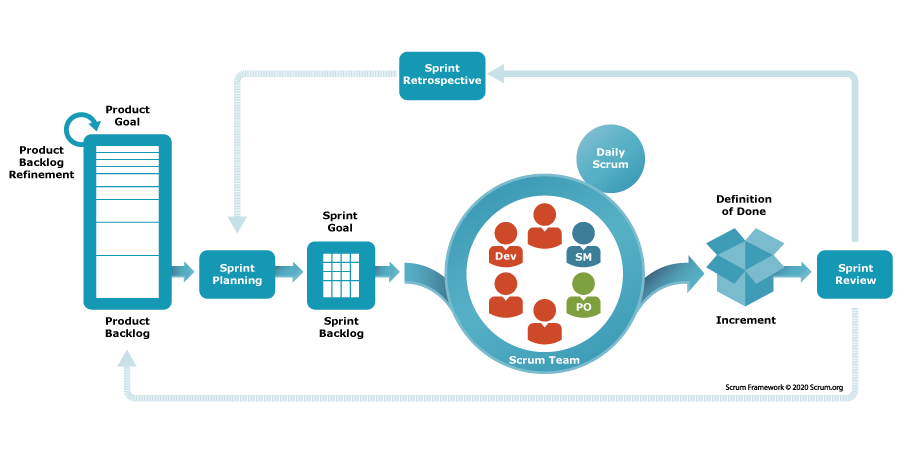
\includegraphics[width=0.42\textwidth]{figures/scrum.png}
\caption{Cyclic representation of Scrum methodology\cite{scrum}}
\label{fig:scrum}
\end{figure}
\FloatBarrier

%----------------------------------------------
\subsection{Application of GIMSI to Business Intelligence}

GIMSI (G\'{e}n\'{e}rer des Indicateurs de performance pour le Management Strat\'{e}gique de
l'Information) guarantees that each KPI selected for the ATB dashboards is aligned with the
strategic objectives of the organization. It ensures the BI solution is a genuine
decision-support instrument, not merely a technical deliverable.

Table~\ref{tab:gimsi_application} presents the application of GIMSI to the ATB Streamlit
dashboard.

\begin{table}[H]
\small
\centering
\caption{Application of the GIMSI methodology to the ATB Streamlit Dashboard}
\label{tab:gimsi_application}
\begin{tabular}{|p{3.5cm}|p{10cm}|}
\hline
\rowcolor{blue!15}
\textbf{GIMSI Phase} & \textbf{Application in the ATB Project} \\
\hline
Needs Analysis & Identification of KPIs for the \textit{Direction March\'{e} Entreprises}: agency performance, client risk, objective tracking \\
\hline
Design & Wireframing of dashboard pages: global overview, risk analysis, agency performance, client segmentation \\
\hline
Development & Streamlit implementation with Plotly visualizations and SQL Server connection \\
\hline
Deployment & Production release of the interactive multi-page dashboard for ATB managers \\
\hline
\end{tabular}
\end{table}
\FloatBarrier

\bigskip

Figure~\ref{fig:gimsi-dashboard} illustrates the general architecture of a GIMSI-based
decision-making information system, as applied to the ATB dashboard design.

\begin{figure}[H]
\centering
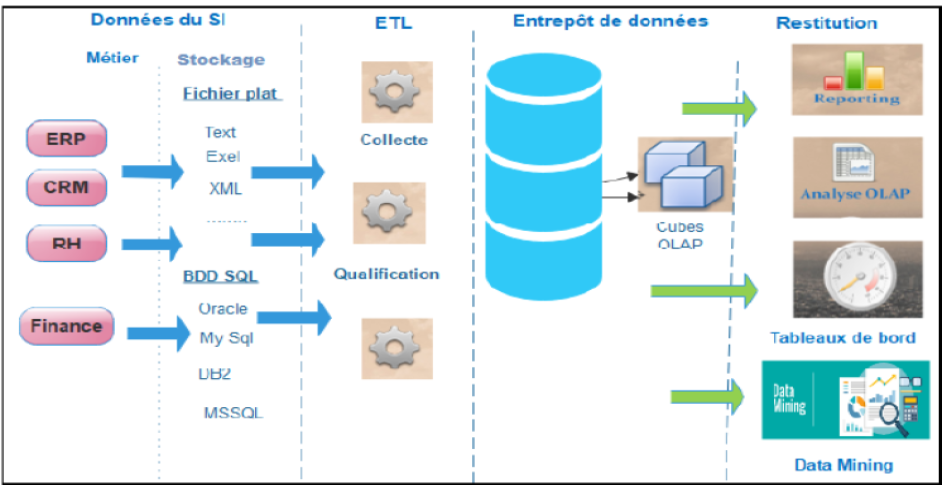
\includegraphics[width=0.8\textwidth]{gimsi.png}
\caption{Architecture of a GIMSI-based decision-support system\cite{gimsi}}
\label{fig:gimsi-dashboard}
\end{figure}
\FloatBarrier

%----------------------------------------------
% GANTT DIAGRAM
%----------------------------------------------

Figure~\ref{fig:gantt_atb} presents the Gantt chart synchronizing the three Releases, the
three Sprints, and the three methodologies of the ATB BI project across 12 weeks.

\begin{figure}[H]
\centering
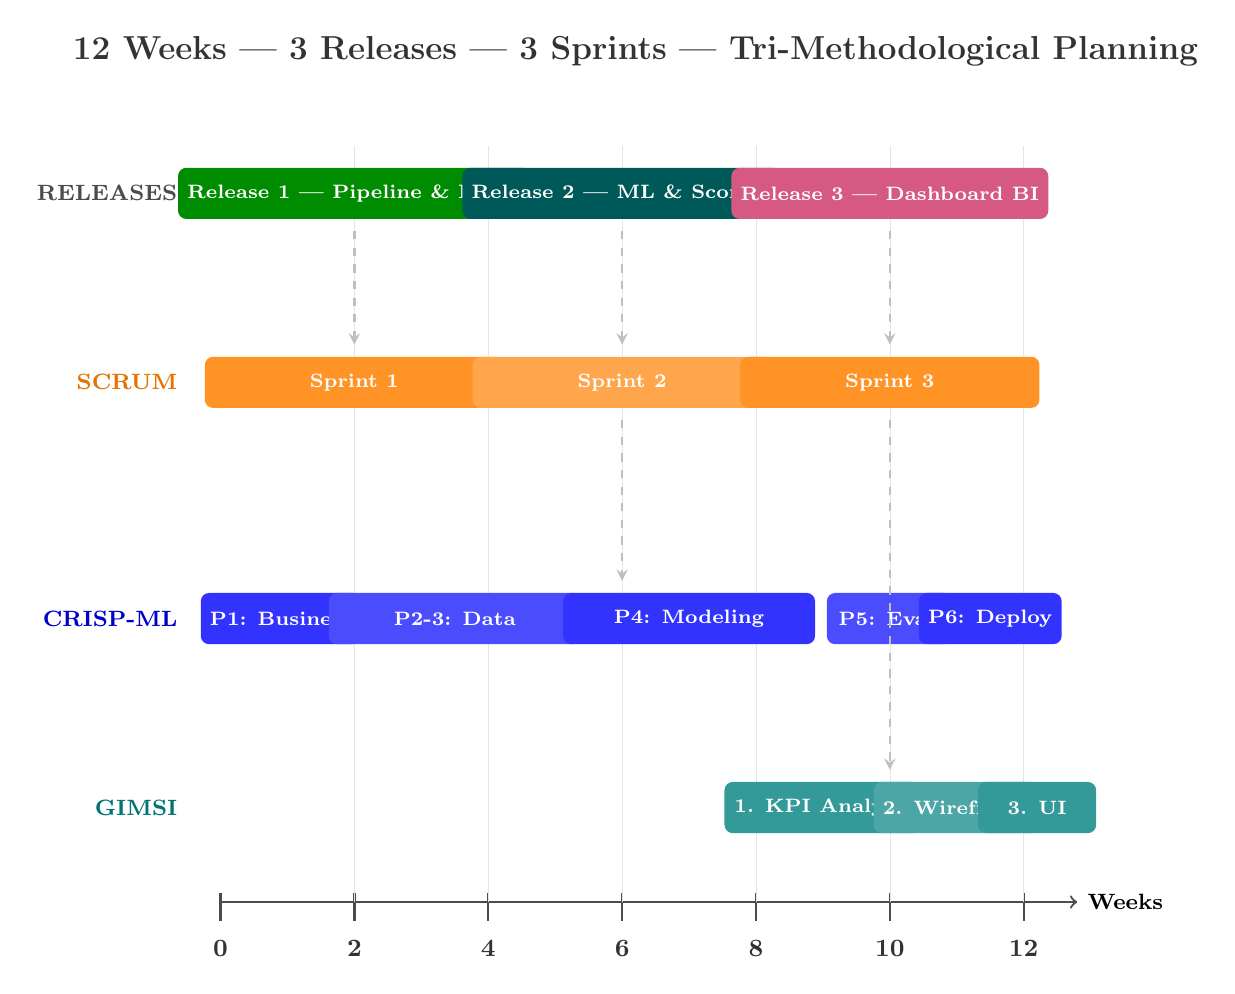
\begin{tikzpicture}[
    xscale=0.85,
    yscale=1.2,
    every node/.style={font=\scriptsize},
    barre/.style={rectangle, rounded corners=3pt, minimum height=0.65cm, text centered,
                  text=white, font=\bfseries\scriptsize},
    trait/.style={thick, gray!50, dashed, -stealth}
]

% WEEK AXIS (12 weeks)
\draw[->, thick, draw=black!70] (0,0) -- (12.8,0)
    node[right, font=\bfseries\footnotesize] {Weeks};
\foreach \x in {0,2,4,6,8,10,12} {
    \draw[thick, draw=black!70] (\x, 0.1) -- (\x,-0.2);
    \node[below, font=\bfseries\small, text=black!80] at (\x,-0.3) {\x};
}
\foreach \x in {2,4,6,8,10,12} {
    \draw[very thin, gray!20] (\x,0) -- (\x,8.0);
}

% RELEASES
\node[anchor=east, font=\bfseries\footnotesize, text=black!70] at (-0.5,7.5) {RELEASES};
\node[barre, fill=green!55!black, minimum width=4.0cm]
    at (2,  7.5) {Release 1 --- Pipeline \& DWH};
\node[barre, fill=teal!70!black,  minimum width=4.0cm]
    at (6,  7.5) {Release 2 --- ML \& Scoring};
\node[barre, fill=purple!65,      minimum width=4.0cm]
    at (10, 7.5) {Release 3 --- Dashboard BI};

% SCRUM
\node[anchor=east, font=\bfseries\footnotesize, text=orange!90!black] at (-0.5,5.5) {SCRUM};
\node[barre, fill=orange!85, minimum width=3.8cm] at (2,  5.5) {Sprint 1};
\node[barre, fill=orange!70, minimum width=3.8cm] at (6,  5.5) {Sprint 2};
\node[barre, fill=orange!85, minimum width=3.8cm] at (10, 5.5) {Sprint 3};

% CRISP-ML
\node[anchor=east, font=\bfseries\footnotesize, text=blue!80!black] at (-0.5,3.0) {CRISP-ML};
\node[barre, fill=blue!80, minimum width=1.6cm] at (0.9, 3.0) {P1: Business};
\node[barre, fill=blue!70, minimum width=3.2cm] at (3.5, 3.0) {P2-3: Data};
\node[barre, fill=blue!80, minimum width=3.2cm] at (7,   3.0) {P4: Modeling};
\node[barre, fill=blue!70, minimum width=1.6cm] at (10,  3.0) {P5: Eval.};
\node[barre, fill=blue!80, minimum width=1.6cm] at (11.5,3.0) {P6: Deploy};

% GIMSI
\node[anchor=east, font=\bfseries\footnotesize, text=teal!90!black] at (-0.5,1.0) {GIMSI};
\node[barre, fill=teal!80, minimum width=2.5cm] at (9,    1.0) {1. KPI Analysis};
\node[barre, fill=teal!70, minimum width=1.8cm] at (11,   1.0) {2. Wireframe};
\node[barre, fill=teal!80, minimum width=1.5cm] at (12.2, 1.0) {3. UI};

% ARROWS
\draw[trait] (2,  7.1) -- (2,  5.9);
\draw[trait] (6,  7.1) -- (6,  5.9);
\draw[trait] (10, 7.1) -- (10, 5.9);
\draw[trait] (10, 5.1) -- (10, 1.4);
\draw[trait] (6,  5.1) -- (6,  3.4);

% TITLE
\node[font=\bfseries\large, text=black!80] at (6.2, 9.0)
    {12 Weeks --- 3 Releases --- 3 Sprints --- Tri-Methodological Planning};

\end{tikzpicture}
\caption{Gantt chart: 3 Releases, 3 Sprints, and 3 methodologies of the ATB BI project
         over 12 weeks.}
\label{fig:gantt_atb}
\end{figure}

%================================================
\section{Conclusion}

This chapter has established the general framework of the project. The presentation of the
Arab Tunisian Bank (ATB)  its history, market segments, organizational structure,
missions, and branch network provides the institutional context within which this
internship was conducted.

The analysis of ATB's current data management process within the \textit{Direction March\'{e}
Entreprises} has highlighted its significant limitations: a manual, error-prone, and
non-scalable Excel-based reporting workflow that hinders rapid and informed strategic
decision-making.

The comparative study of existing approaches (the internal Excel-based process and the
Power BI platform) confirmed the absence of a solution that simultaneously integrates
automated data collection, governed transformation, predictive intelligence, and fully
customizable interactive dashboards within an open-source, cost-free architecture.

Finally, a rigorous tripartite methodological architecture has been defined and
justified: Scrum as the global project management framework, CRISP-ML to
guide data engineering and machine learning pipeline development, and GIMSI to
orient the design of decision-support dashboards for ATB management.

The following chapter presents the state of the art of the technical domains mobilized for
the design of this Business Intelligence and Machine Learning platform.
